\section{Disturbance observer}
\begin{frame}
    \frametitle{Outline}
    \tableofcontents[currentsection]
\end{frame}

\begin{frame}
    \frametitle{Disturbance Observer}

    The following control structure is referred to as a disturbance observer:
    \begin{figure}
        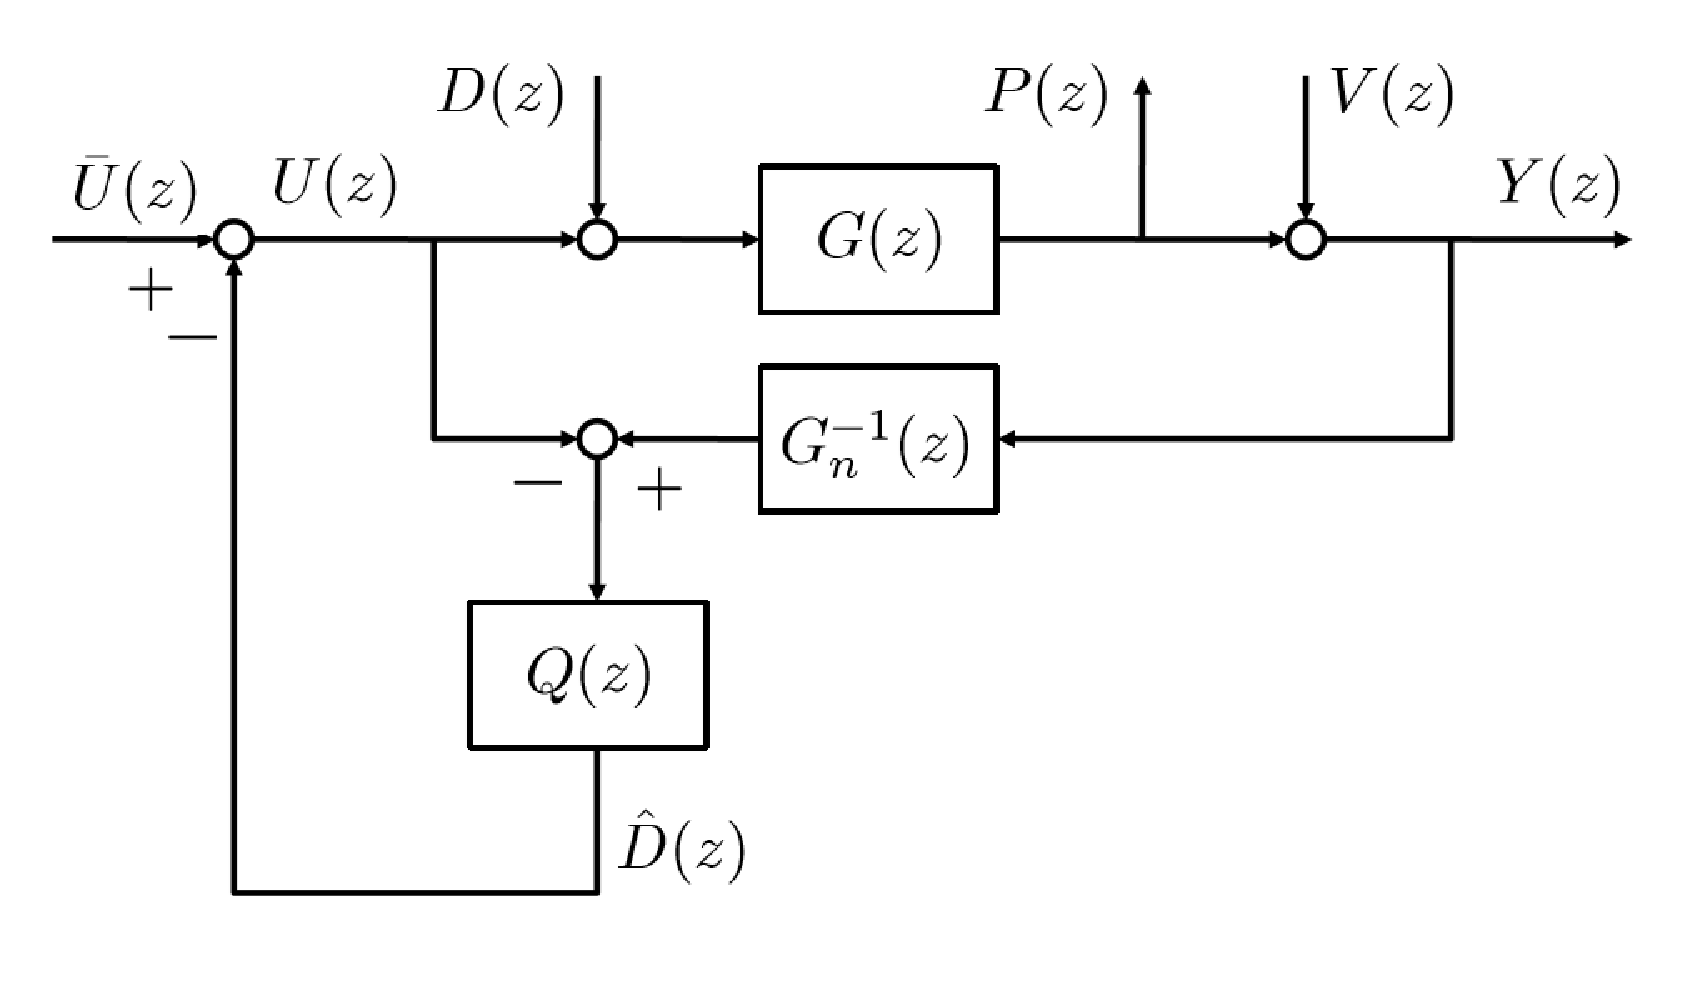
\includegraphics[width=0.7\textwidth]{Disturbance_Observer_DO}\\
    \end{figure}

    The signals are:

    \begin{center}
    \begin{tabular}{l @{ : } lll @{ : } l}
        $U(z)$ & control input && $V(z)$ & measurement noise \\
        $D(z)$ & disturbance && $\hat{D}(z)$ & estimate of $D(z)$ \\
        $Y(z)$ & measured output && $P(z)$ & performance output
    \end{tabular}
    \end{center}
\end{frame}

\begin{frame}
    \frametitle{Disturbance Observer}

    \begin{figure}
        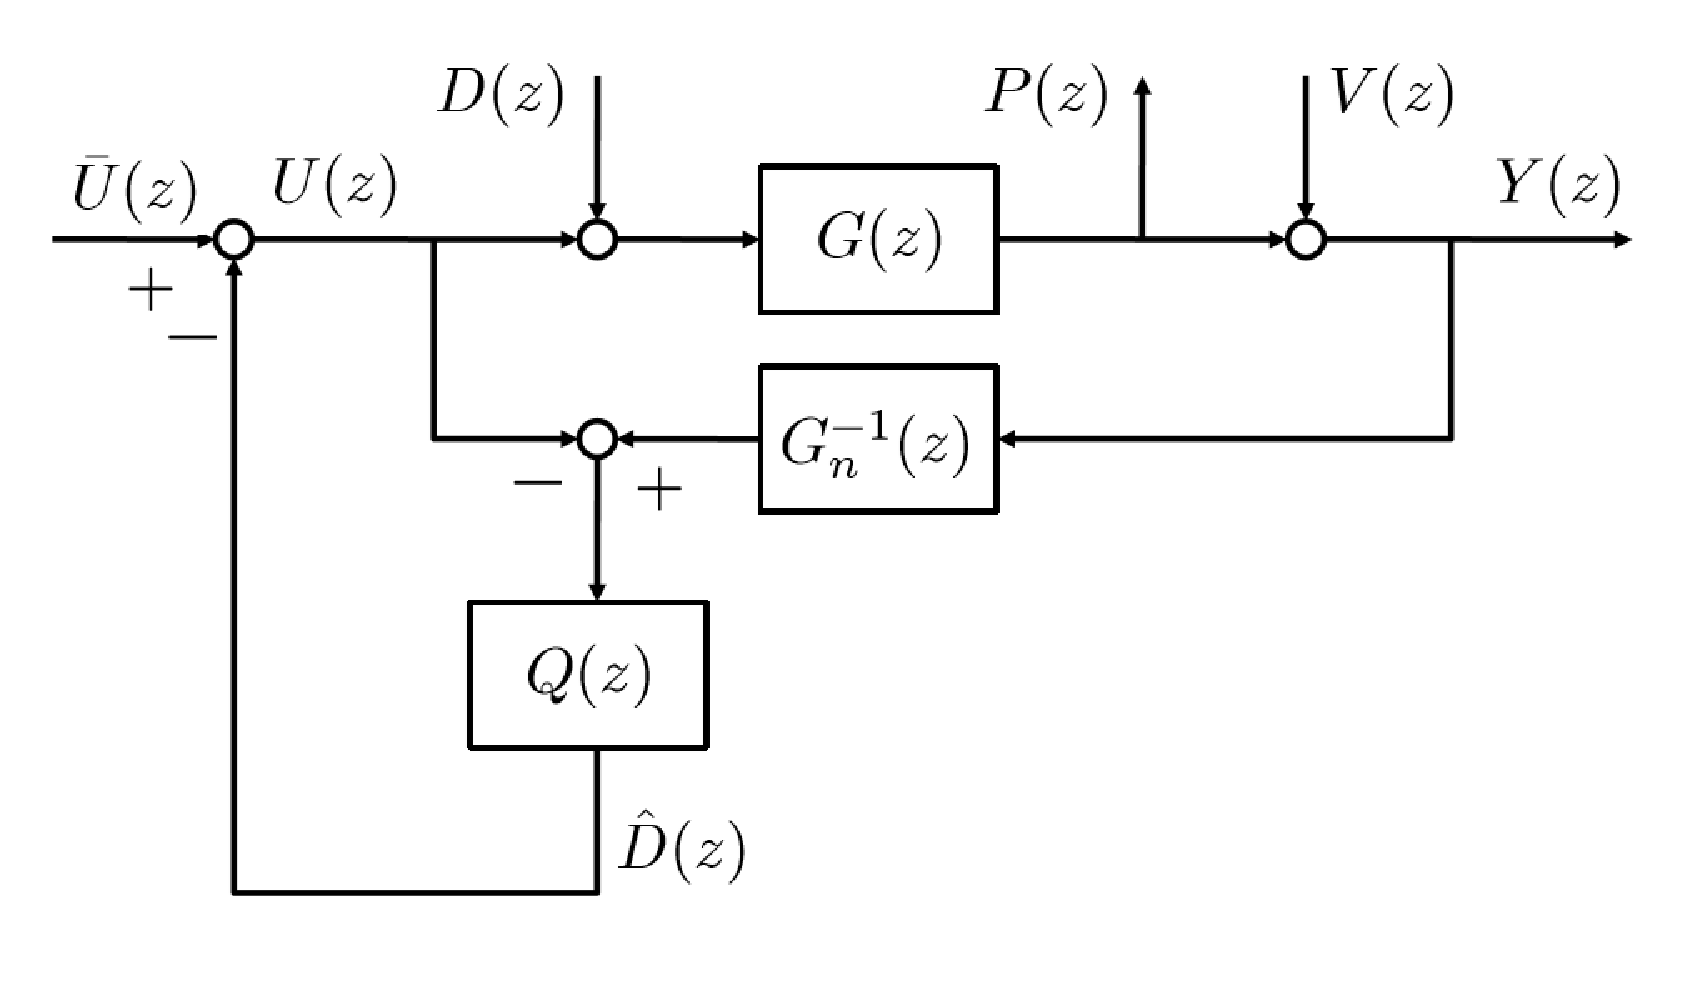
\includegraphics[width=0.7\textwidth]{Disturbance_Observer_DO}\\
    \end{figure}

    \begin{itemize}
    \item
    The one difference in the control architecture (compared to the motivation) is the presence of $Q(z)$

    \item
    $Q(z)$ is used to make the dynamics from $U(z)$ and $Y(z)$ to $\hat{D}(z)$ realizable
    \end{itemize}
\end{frame}

\begin{frame}
    \frametitle{Disturbance Observer---Comparison to Motivation}

    \begin{figure}
        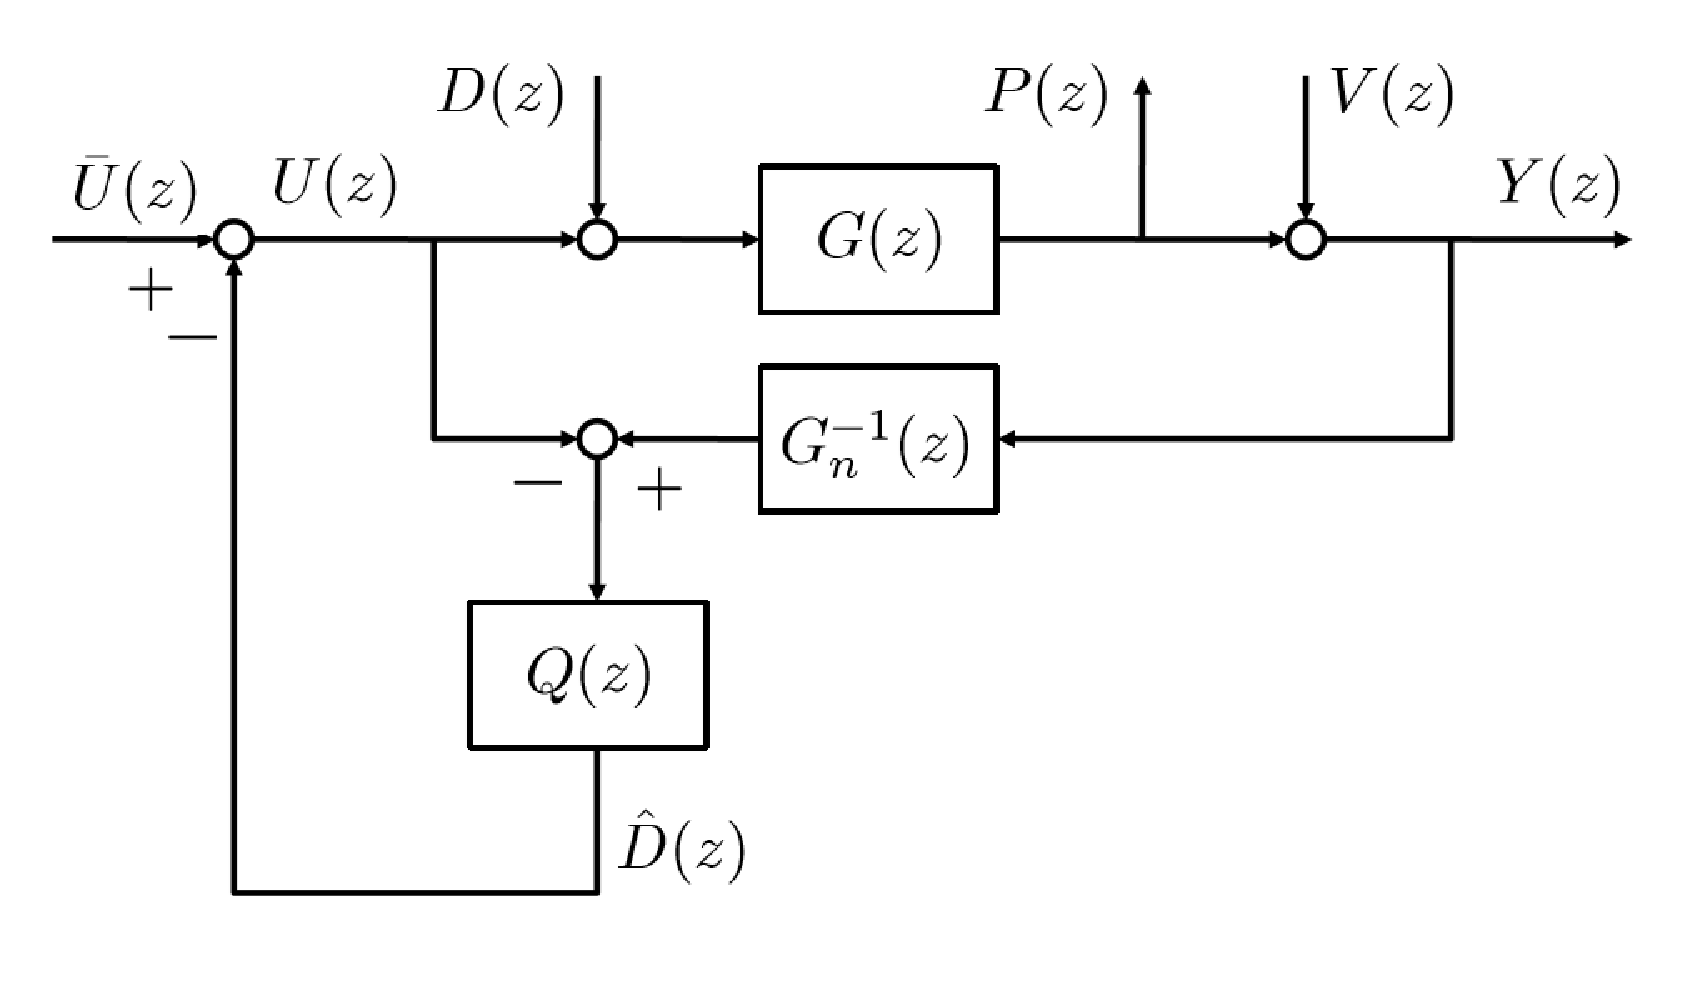
\includegraphics[width=0.7\textwidth]{Disturbance_Observer_DO}\\
    \end{figure}

    The structure in the Motivation section corresponds to
    \begin{itemize}
    \item
    $G(z) = G_n(z)$ (the plant is exactly as modeled)
    \pause

    \item
    $V(z) = 0$ (there is no sensor noise)
    \pause

    \item
    $Q(z) = 1$ (it is possible to realize $G_n^{-1}(z)$ )

    \end{itemize}
\end{frame}


